


Geomecânica é o estudo das deformações e tensões em solos e rocha. Esse estudo se torna de extrema importância, pois, várias problemas podem ser solucionados através desses estudos, como:
\begin{itemize}
    \item Cálculo da pressão de fratura.
    \item Estabilidade de poços
\end{itemize}

Assim, simulações de geomecânicas são importantes para uma exploração segura do campo.

\section{Tensor de Tensões}

Para representar a tensão em um ponto da rocha, é utilizado um tensor de tensões de segunda ordem como segue abaixo:

\begin{equation}
\mathbf{\sigma} =
    \begin{bmatrix}
    \stxx & \stxy & \stxz \\
    \styx & \styy & \styz \\
    \stzx & \stzy & \stzz
    \end{bmatrix}
\end{equation}

O primeiro subscrito do tensor representa a face que a tensão está sendo aplicada, enquanto o segundo representa a direção da tensão. A figura \ref{fig:tensoesx} mostra as componentes com o com primeiro subscrito x.


\begin{figure}[!htbp]
\centering
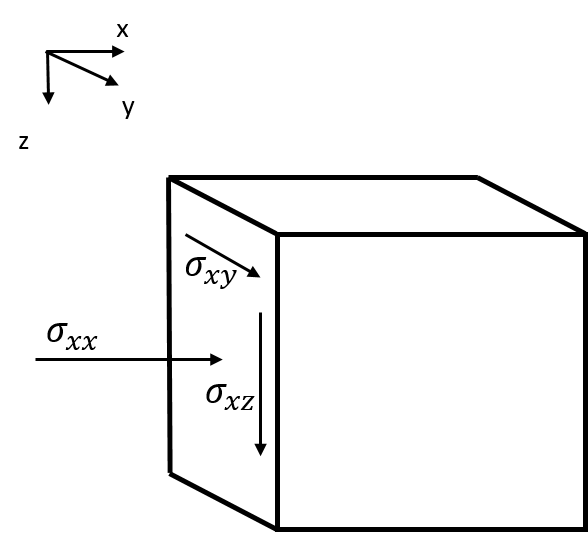
\includegraphics[width=5cm]{chap01/tensor.png}
\caption{Tensões $\sigma_{x.}$ representadas graficamente.}
\label{fig:tensoesx}
\end{figure}

Ao aplicar a condição de equilíbrio do momento, chega-se a conclusão que $\stxy=\styx$, $\stxz=\stzx$ e $\styz=\stzy$. Dessa maneira, para a representação desse tensor, são necessários guardar apenas seis valores. Dessa forma, pode-se considerar a tensão como o vetor apresentado \label{eq:tensor6} essa notação é chamada de notação de Voigt e é a bastante utilizada nas implementações de elementos finitos, por exemplo, nas formulações apresentadas por \cite{hughes} e \cite{jacob}.


\begin{equation}
\sigma^T = \begin{bmatrix}
\stxx & \styy & \stzz & \stxy & \stxz & \styz
\end{bmatrix}
\label{eq:tensor6}
\end{equation}


\section{Teoria da Consolidação}

Para um certo elemento de volume $\Delta x\Delta y \Delta z$, representado na figura \ref{fig:equilibrio}, pode-se escrever o equilíbrio nas direções x, y e z.

\begin{figure}[!htbp]
\centering
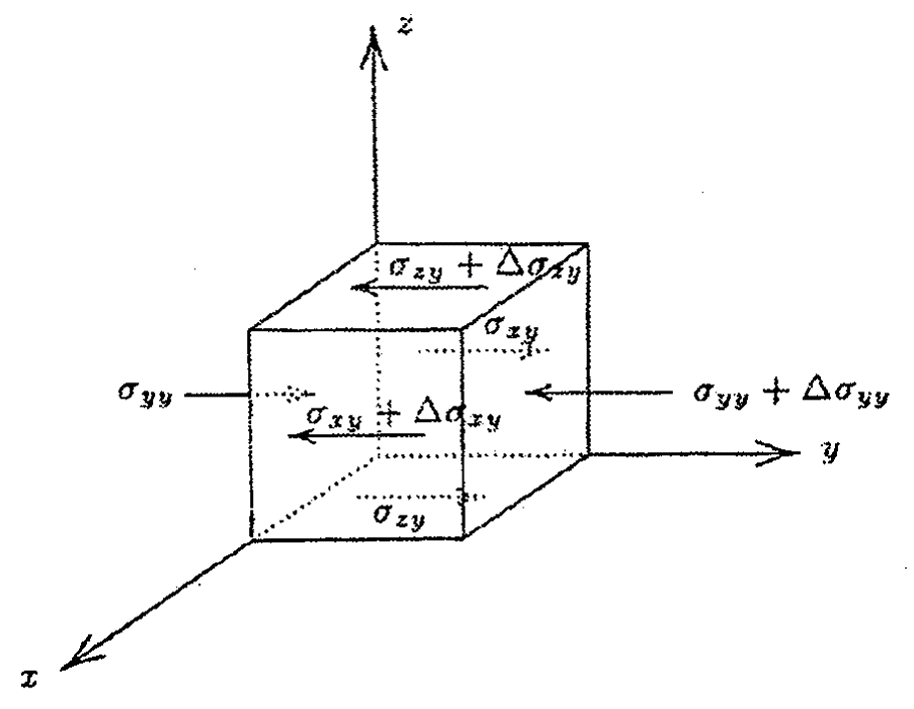
\includegraphics[width=6cm]{chap01/equilibrio.png}
\caption{Tensões na direção y ($\sigma_{.y}$) representadas graficamente.  Fonte: \cite{CompGeomec}}
\label{fig:equilibrio}
\end{figure}

Para a direção y, por exemplo, tem-se:

\begin{multline}
   (\stxy - \stxy - \Delta \stxy) \Dy\Dz + (\styy - \styy - \Delta \styy)\Dx\Dz  +\\
   + (\stzy - \stzy - \Delta\stzy) \Dx\Dy + f_y\Dx\Dy\Dz = 0
\end{multline}

\begin{equation}
 \Delta \stxy \Dy\Dz + \Delta \styy\Dx\Dz + \Delta\stzy - f_y\Dx\Dy\Dz = 0
\end{equation}

\begin{equation}
\dx[\stxy] + \dy[\styy] + \dy[\stzy] - f_y = 0
\end{equation}

Analogamente, para as outras direções, pode-se montar o seguinte sistema de equações de equilíbrio.

\begin{equation}
\label{eq:equilibrio1}
\left\{\begin{matrix}
 \dx[\stxx] + \dy[\styx] + \dz[\stzx] - f_x & = & 0\\
 \dx[\stxy] + \dy[\styy] + \dz[\stzy] - f_y & = & 0\\
 \dx[\stxz] + \dy[\styz] + \dz[\stzz] - f_z & = & 0
\end{matrix}\right.
\end{equation}

As tensões apresentadas nas equações \ref{eq:equilibrio1} são as atuam no bloco infinitesimal. Acontece que ao tratar de reservatórios de petróleo, estes possuem fluído no volume poroso da rocha (óleo ou água) e, portanto, parte da tensão será suporta pelo fluído e parte será suportado pelos grãos da rocha. Como fluído não oferece resistência ao cisalhamento, ele suporta apenas parte das tensões $\stxx$, $\styy$ e $\stzz$.

Experimentalmente foi constado por Biot em que a equação que rege a tensão efetiva na rocha ($\sigma^{\prime\prime}$) é dada pela equação \ref{eq:tensaoefetiva} (veja \cite{ResGeomec} cap 02).

\begin{equation}
\label{eq:tensaoefetiva}
    \sigma^{\prime\prime} = \sigma - \alpha P_p
\end{equation}

Onde $\alpha$ é o coeficiente de biot e $P_p$ a pressão de poros. O coeficiente de biot representa o quanto a pressão de poros do fluído suporta a tensão total na rocha, portanto, $\alpha \in [0,1]$.

Assim, as equações \ref{eq:equilibrio1} podem ser reescritas como \ref{eq:equilibrio} substituindo a tensão total $\sigma$ pela tensão efetiva na rocha ($\sigma^\prime$). Essas equações são encontras em \cite{CompGeomec}.



\begin{equation}
\label{eq:equilibrio}
\left\{\begin{matrix}
\dx[\sxx]  + \dy[\syx] + \dz[\szx] + \dx[\alpha P_p] - f_x   = 0
\\
\dx[\sxy]  + \dy[\syy] + \dz[\szy] + \dy[\alpha P_p]  - f_y   = 0
\\
\dx[\sxz]  + \dy[\syz] + \dz[\szz] + \dz[\alpha P_p] - f_z   = 0
\end{matrix}\right.
\end{equation}

Ou ainda, escrevendo de forma matricial.

\begin{equation}
\label{eq:equilibrio_matriz}
\nabla \cdot \sigma^\prime + \nabla \alpha P_p - f = 0
\end{equation}

Onde $f^T=\begin{bmatrix}f_x & f_y & f_z\end{bmatrix}$.


Por motivos de implementação mais eficiente menor uso de memória e utilização de operações mais simples (multiplicação de matrizes por vetores) a equação acima pode ser escrita na notação de Voigt que considerando as definições abaixo:

\begin{equation}
\begin{matrix}
\sigma^\prime = \begin{bmatrix}
\sxx
\\
\syy
\\
\szz
\\
\sxy
\\
\sxz
\\
\syz
\end{bmatrix}
&

;

&

f = \begin{bmatrix}
f_{x}
\\
f_{y}
\\
f_{z}
\end{bmatrix}
&
;
&

m = \begin{bmatrix} 1 \\ 1 \\ 1 \\ 0 \\ 0 \\ 0\end{bmatrix}

&
;

&
\sopnabla = \sop
\end{matrix}
\end{equation}

A equação \ref{eq:equilibrio_matriz} pode ser reescrita como \ref{eq:equilibrio_final}.

\begin{equation}
\label{eq:equilibrio_final}
\sopnabla^T\sigma^\prime + \sopnabla^T\alpha m  P_p - f = 0
\end{equation}


\subsection{Relações Constitutivas}

\textit{"Uma relação constitutiva descreve a deformação de uma rocha em resposta a uma tensão (e vice-versa)."} \cite{ResGeomec}


Vários tipos de leis constitutivas podem ser utilizadas para representar essa relação entre tensão e deformação. A figura \ref{fig:stress_strain} mostram dados de um teste típico de tensão-deformação em uma rocha bem cimentada. Nesse caso, é importante notar que o comportamento linear é a região dominante nesse tipo de teste. Essa região onde as deformações e tensões se relacionam linearmente é chamada de elástica.


\begin{figure}[!htbp]
\centering
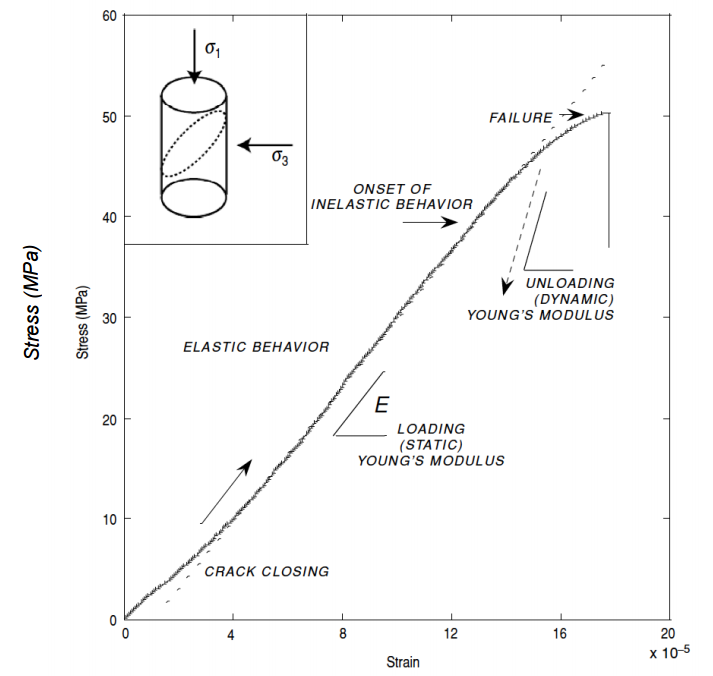
\includegraphics[width=7cm]{chap01/stress_strain.PNG}
\caption{Teste de laboratório tensão-deformação para uma rocha bem cimentada. Fonte: \cite{ResGeomec}}
\label{fig:stress_strain}
\end{figure}


O estudo de mecânica dos sólidos nos mostra que, na região elástica e materiais isotrópicos, é possível escrever uma relação entre as deformações e tensões nos elementos de forma simples. Essa relação é denominada de Lei de Hooke Generalizada e é apresentada na Equação \eqref{eq:hooke}. E a Equação \eqref{eq:elasticMatrix} apresenta a matriz de elasticidade.


\begin{equation}{
\label{eq:hooke}
\fontsize{4}{4}\selectfont
\sigma ^{\prime\prime}= D \epsilon
}
\end{equation}



Onde $E$ é o módulo de Young da rocha e $v$ o módulo de de Poisson. Já as deformações se relacionam com os deslocamentos pela equação \eqref{eq:defor_desloc}.

\begin{equation}
\label{eq:defor_desloc}
\epsilon = \sopnabla u
\end{equation}


A EDP da equação \eqref{eq:equilibrio_final} pode então ser escrita em função dos deslocamentos substituindo as equações \eqref{eq:hooke} e \eqref{eq:defor_desloc}.

\begin{equation}
\label{eq:edp_geomec}
\sopnabla^TD \sopnabla u + \sopnabla^T\alpha m P_p - f = 0
\end{equation}

Onde $D$ é a matriz de elasticidade da Lei de Hooke. Essa forma será a utilizada junto dos métodos do elementos finitos para construção de um simulador para regime permanente de geomecânica em duas dimensões. Ao se passar
de três dimensões para duas dimensões existem duas abordagens possíveis de stress plano ou deformação plana. Que são apresentadas respectivamente em \eqref{eq:elasticplanestress} e \eqref{eq:elasticplanestrain}.

\begin{equation} \label{eq:elasticplanestress}
D_{stress} = \frac{E}{1-\upsilon^2}
\begin{bmatrix}
1  & \upsilon & 0 \\ 
\upsilon & 1 &  0 \\ 
0 & 0 & \frac{1-\upsilon}{2}
\end{bmatrix}
\end{equation}

\begin{equation} \label{eq:elasticplanestrain}
D_{strain} = \frac{E}{(1+\upsilon)(1-2\upsilon)}
\begin{bmatrix}
 1-\upsilon & \upsilon    &  0 \\ 
 \upsilon   &  1-\upsilon &  0 \\ 
 0& 0 & \frac{1-2\upsilon}{2}
\end{bmatrix}
\end{equation}

De acordo com \cite{jacob}, a condição de deformação plana é melhor aplicada quando o elemento é grosso em relação ao plano xy que é o caso dos reservatórios de petróleo.  Dessa forma, artigos como \cite{planeStrainProblems}, \cite{casteletto} e \cite{irina} utilizam a hipótese de deformação plana que será a mesma utilizada nesse trabalho.

Os operadores e vetores devem então ser redefinidos para os mostrados em \eqref{eq:vetores2d}.

\begin{equation}
\label{eq:vetores2d}
\begin{matrix}
\sigma^\prime = \begin{bmatrix}
\sxx
\\
\syy
\\
\sxy
\end{bmatrix}
&

;

&

f = \begin{bmatrix}
f_{x}
\\
f_{y}
\end{bmatrix}
&
;
&

m = \begin{bmatrix} 1 \\ 1 \\ 0\end{bmatrix}

&
;

&
\sopnabla = \soptwod

&
;

&

u = \begin{bmatrix}
u_x
\\ 
u_y
\end{bmatrix}

\end{matrix}
\end{equation}

Além da Equação \eqref{eq:edp_geomec}, são necessárias as condições de contorno para que o problema fique totalmente definido. 

\section{Modelagem pelo Método dos Elementos Finitos}

Em posse da Equação \eqref{eq:edp_geomec}, é necessário um método de solução numérica para se resolver. O método utilizado nesse trabalho é o método dos Elementos Finitos. O método dos Elementos finitos é bastante difundido em análises estruturais mas também pode ser utilizado em outros tipos de EDP's como fluxo de calor. 



\subsection{Formulação Fraca}

O primeiro passo para utilizar o método dos elementos finitos é chegar na formulação fraca da equação \eqref{eq:edp_geomec}. As referências \cite{jacob} e \cite{hughes} mostram a dedução para chegar em  \eqref{eq:weakform}.

\begin{equation}\label{eq:weakform}
\omeint{ (\sopnabla \mathbf{w})^T D \sopnabla  \mathbf{u}} - \int_{\Gamma_\sigma} \mathbf{w} \bar{\mathbf{t}} d\Gamma = 0 \quad \forall \mathbf{w} \in \trial 
\end{equation}


Com conjunto de teste $\trial = \trialdef$ e conjunto de avaliação igual a $\test = \testdef$.




\subsection{Divisão do domínio}

O domínio do problema será dividido em uma quantidade finita de elementos, o conjunto desses elementos será chamado de $\Tau^h$.  A partição do domínio será realizada em elementos quadriláteros apesar de outras tipos de elementos estarem disponíveis (por exemplo, elementos triangulares). A figura \ref{fig:elemento} mostra como serão os elementos que dividirão o domínio.

%TODO trocar por figura em que os elementos não sejam 
\begin{figure}[!htbp]
\centering

\includegraphics[width=5cm]{interrogacao.png}
\caption{Exemplo de domínio dividido em quadriláteros.}
\label{fig:elemento}
\end{figure}

A notação utilizada aqui é a mesma que em \cite{casteletto} para manter a coerência com o Capítulo \ref{ch:multiescala}. Para esse tipo de elemento a quantidade de vértices é quatro. Como o campo aproximado de deslocamentos está no plano xy, cada vértice terá dois graus de liberdade um na direção x e um na direção y, que de maneira indistinta serão chamados de $d_i^h$ para algum $i$ que são as variáveis a serem descobertas para encontrar a solução $\textbf{u}$ aproximada. A quantidade de graus de liberdade será chamada de $\freedomfine$. Um nó pertencente a fronteira de $\Omega$  já tem seu grau de liberdade determinado e, portanto, não será uma variável do problema e esses valores serão chamados de $\bar{d}_i^h$ a quantidade de graus de liberdade pertencentes a fronteira de dirichlet será chamada de $\essentialfine$.  Assim, o campo vetorial $u$ será aproximado através de funções $ \basefunctionfine : \Omega \rightarrow \mathbb{R}^2 \quad \forall \quad i=1,2,...,\freedomfine$  relativa aos graus de liberdade e  $ \basefunctionfine : \Omega \rightarrow \mathbb{R}^2 \quad \forall \quad i=\freedomfine+1,2,...,\freedomfine + \essentialfine$  relativas as condições de contorno de Dirichlet através de \eqref{eq:udiscret}.


\begin{equation}\label{eq:udiscret}
\mathbf{u}(\mathbf{x}) = \sum_{i=1}^{\freedomfine} \basefunctionfine  d_i^h + {\sum_{i=1}^ {n^h_{\bar{u}}}}  \basefunctionfineessential \bar{d}_i^h = \mathbf{N^h} \mathbf{d}^h + \mathbf{\bar{N}^h} \mathbf{\bar{d}}^h
\end{equation}

onde 

\begin{eqnarray*}
\mathbf{N^h} = [N^h_1, N^h_2, ..., N^h_{\freedomfine} ] \\
\mathbf{\bar{N}^h}  =[N^h_{\freedomfine + 1}, N^h_{\freedomfine + 2}, ..., N^h_{\freedomfine + \essentialfine}] \\
\mathbf{d} = [d_1^h, d_2^h, ... , d_{\freedomfine}^h]^T \\
\bar{\mathbf{d}} = [\bar{d}_1^h, \bar{d}_2^h, ... , \bar{d}_{\essentialfine}^h]^T
\end{eqnarray*}



Por enquanto, as funções $N^h_i$ em uma abordagem clássica de elementos finitos, serão da forma $[N^h_{ix} \quad 0]^T$ para um grau de liberdade x e  $[0 \quad N^h_{iy}]^T$  para um grau de liberdade y, dessa forma, um grau de liberdade x não é utilizado para interpolar o valor do campo $u_y(x, y)$ e vice-versa. De acordo com \cite{jacob} essa é a forma mais usual, porém, é possível utilizar outras opções. De fato, a funções de forma que serão utilizadas no método multiescala que serão apresentadas em \ref{ch:multiescala} não vão obedecer esse padrão . A forma exata da definição será apresentada mais a frente pois elas serão definidas em um sistema diferente do (x,y). Agora as funções $N^h_{ix}$ e $N^h_{iy}$ são tais que os valores tem valor igual a um no seu nó correspondente e possuem valor zero em todos os outros nós, mais especificamente, o suporte dessas funções são apenas os elementos que possuem o nó correspondente como vértice. Um exemplo dessas funções é apresentado na Figura \ref{fig:shapefunctions}

\begin{figure}[h]
\center
\subfigure[ Numeração global dos nós em malha $3\times3$. Marcados de vermelho o nó 6 e seus adjacentes. ]{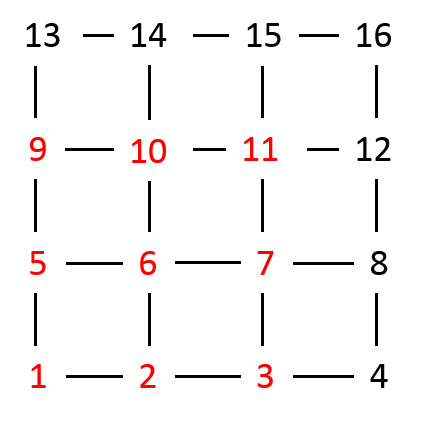
\includegraphics[width=0.45\textwidth]{chap01/figs/grid3x3ver.png}}\label{fig:grid3x3ver}
\qquad
\subfigure[ Numeração das funções de forma $N_i^h$. Azul as funções de forma relativa à condição de contorno de Dirichlet ]{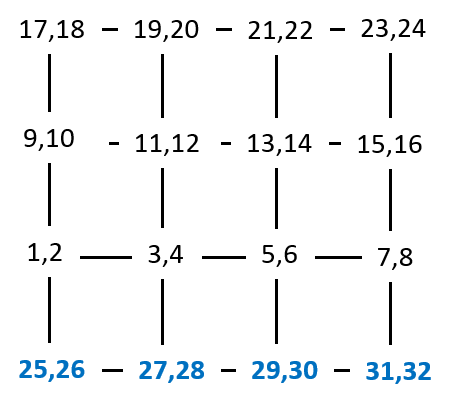
\includegraphics[width=0.45\textwidth]{chap01/figs/grid3x3_Ni.png}}

\caption{Numeração dos nós e das funções de base. Para numeração das funções de base foi considerada a borda inferior com condição de Dirichlet nas direções x e y. }
\end{figure}


\begin{figure}[h]
\center
\subfigure[ ${\basefunctionfine[9x]}$ ou ${\basefunctionfine[10y]}$ ]{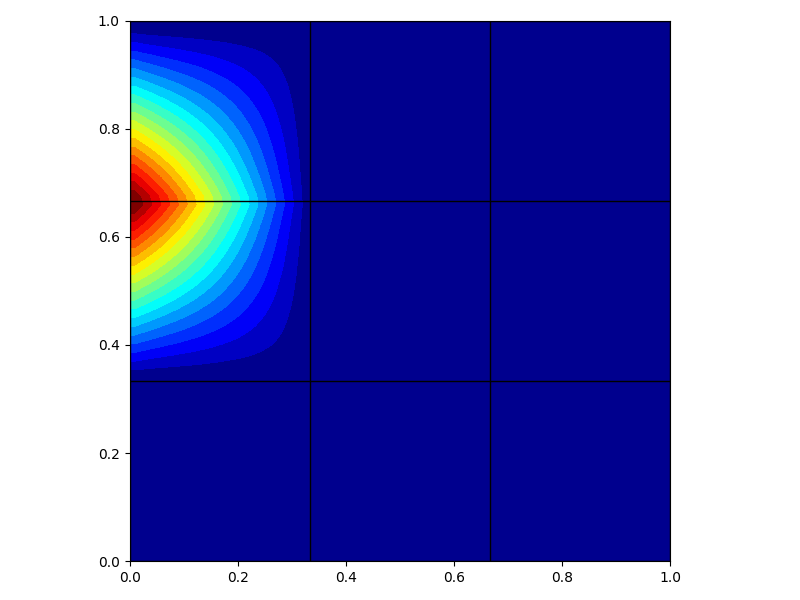
\includegraphics[width=0.45\textwidth]{chap01/figs/prolongation/prolongation_x_total_016.png}}
\qquad
\subfigure[ ${\basefunctionfine[13x]}$ ou ${\basefunctionfine[14y]}$ ]{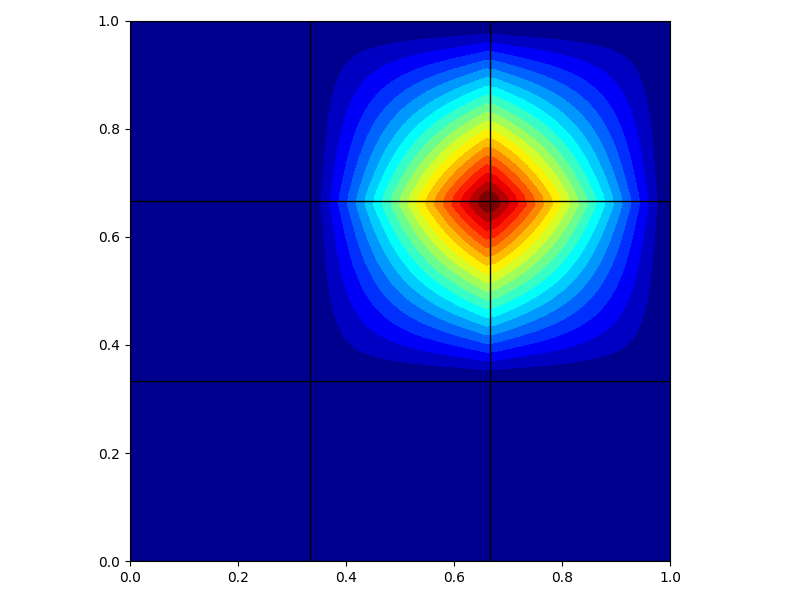
\includegraphics[width=0.45\textwidth]{chap01/figs/prolongation/prolongation_x_total_020.png}}

\subfigure[ ${\basefunctionfine[27x]}$ ou ${\basefunctionfine[28y]}$ ]{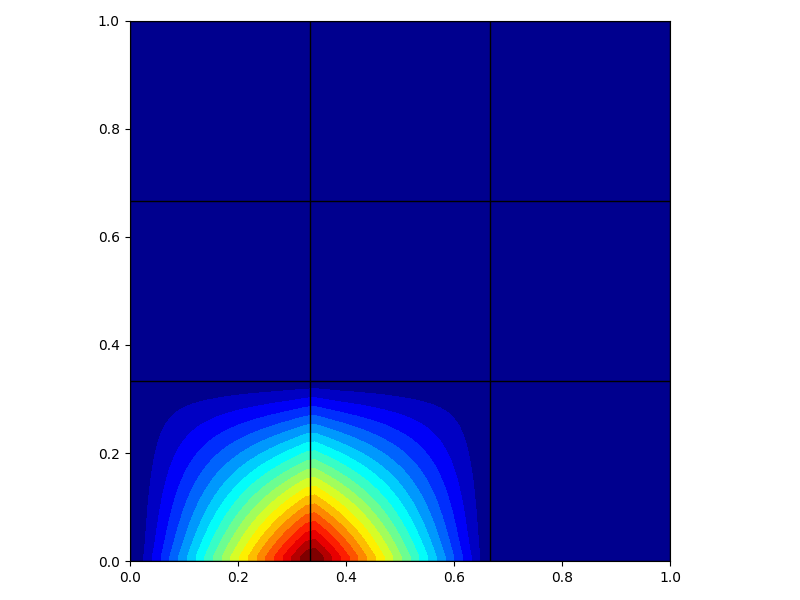
\includegraphics[width=0.45\textwidth]{chap01/figs/prolongation/prolongation_x_total_002.png}}
\qquad
\subfigure[ ${\basefunctionfine[31x]}$ ou ${\basefunctionfine[32y]}$ ]{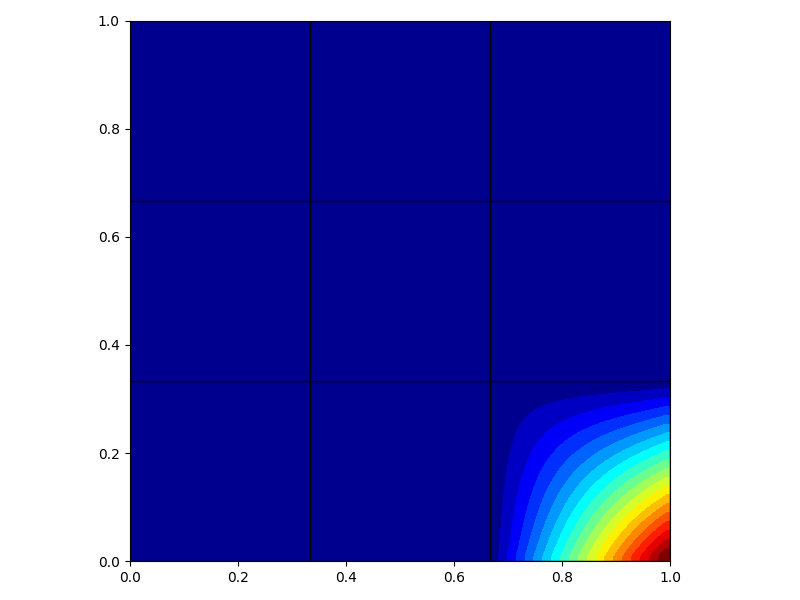
\includegraphics[width=0.45\textwidth]{chap01/figs/prolongation/prolongation_x_total_006.png}}
\caption{Gráficos das funções de forma para um grid 3x3. Foi considerada condição de Dirichlet na fronteira abaixo }\label{fig:shapefunctions}
\end{figure}
    


\subsection{Construção do sistema linear}

Dado a forma fraca definida em \eqref{eq:weakform} e as funções de forma $N_i^h$ para $i = 1, 2, 3, ..., \freedomfine + \essentialfine$ pode-se encontrar uma solução aproximada pelo método de Galerkin. O método consiste em procurar solução não mais para $\mathbf{w} \in \trial$ e $\mathbf{u} \in \test$, mas em encontrar uma solução aproximada nos conjuntos  $\mathbf{w^h} \in \trialaprox = \text{span}\{ \basefunctionfine | i = 1,2, ..., \freedomfine  \}$ e $\mathbf{u}$ da forma aproximada mostrada na \eqref{eq:udiscret} pode-se chegar na forma fraca aproximada \eqref{eq:weakformaprox}.


\begin{equation}\label{eq:weakformaprox}
\omeint{ (\sopnabla \mathbf{w}^h)^T D \sopnabla  \mathbf{u}^h}  =  \int_{\Gamma_\sigma} \mathbf{w}^h \bar{\mathbf{t}} d\Gamma \quad \forall \mathbf{w}^h \in \trialaprox
\end{equation}


Assim, se substituirmos $\mathbf{w}$ por cada uma das funções $N_i^h$ para $i = 1, 2, 3, ..., \freedomfine$ em \eqref{eq:weakformaprox} pode-se obter um conjunto de equações que formam um sistema linear. Seguem abaixo os cálculos substituindo $\mathbf{w}$ por $\basefunctionfine$ e $\mathbf{u}^h$ por \eqref{eq:udiscret}.


\begin{equation}
\omeint{ (\sopnabla \basefunctionfine)^T D \sopnabla (\mathbf{N^h} \mathbf{d}^h + \mathbf{\bar{N}^h} \mathbf{\bar{d}}^h )} = \int_{\Gamma_\sigma} \basefunctionfine \bar{\mathbf{t}} d\Gamma 
\end{equation}

\begin{equation}\label{eq:umaequacaosistema}
\omeint{ (\sopnabla \basefunctionfine)^T D \sopnabla \mathbf{N^h} \mathbf{d}^h }  = \int_{\Gamma_\sigma} \basefunctionfine \bar{\mathbf{t}}  d\Gamma - \omeint{ (\sopnabla \basefunctionfine)^T D \sopnabla  \mathbf{\bar{N}^h} \mathbf{\bar{d}}^h} 
\end{equation}

Definindo, 

\begin{equation}\label{eq:entradamatriz}
    K_{i,j} = \omeint{(\sopnabla \basefunctionfine)^T D \sopnabla \basefunctionfine[j]}
\end{equation}


A primeira parcela do lado esquerdo pode ser reescrita como:

\begin{equation}
     (\sopnabla \basefunctionfine)^T D \sopnabla \mathbf{N^h} = [K_{i,1}\quad  K_{i,2} \quad ... \quad K_{i,\freedomfine}] 
\end{equation}

E definindo o lado direito de \eqref{eq:umaequacaosistema} como $f_i$, pode-se reescrever a equação como:

\begin{equation} \label{eq:umaequacaosistemafim}
K_{i,:} \mathbf{d}^h = f_i \quad \forall \quad i=1,..., \freedomfine
\end{equation}

E finalmente substituindo todos os valores possíveis de $i$ encontrasse o sistema linear \eqref{eq:sistemalinear}.

\begin{equation}
    \mathbf{K} \mathbf{d} = \mathbf{f}
\end{equation}



onde as entradas de $K$ são definidas por  $K_{i,j} = \omeint{\kij{i}{j}}$. A solução do sistema são tem como resultado os valores de cada um dos graus de liberdade do problema e com isso, encontrar a aproximação dos deslocamentos \eqref{eq:udiscret}. Sobre a matriz $\mathbf{K}$ satisfaz as seguintes propriedades:


\begin{itemize}
    \item A matriz é simétrica. Pois,

    \begin{eqnarray}
    K_{i,j} & = & (K_{i,j})^T \\
            & = & \omeint{((\sopnabla \basefunctionfine)^T D \sopnabla \basefunctionfine[j])^T} \\
            & = & \omeint{ ( \sopnabla \basefunctionfine[j])^T D^T  ((\sopnabla \basefunctionfine)^T)^T}\\
            & = & \omeint{ ( \sopnabla \basefunctionfine[j])^T D  (\sopnabla \basefunctionfine)} \\
            & = & K_{j,i}
    \end{eqnarray}


    \item A matriz é esparsa. Pois cada uma das funções de forma é não nula apenas nos elementos em que aquele nó é vértice. No caso de uma malha de quadriláteros, cada função de forma é não nula em quatro elementos apenas.

    \item A matriz é positiva definida. A prova desse fato é encontrada em \cite{hughes}, que mostra que esse propriedade depende da relação constitutiva ser também positiva definida.
\end{itemize}


Ainda sobre a esparsidade da matriz de rigidez, em um grid com quadriláteros cada função de base de um nó (a menos de nós de fronteira) tem conexão com nove outros nós, contando com ele mesmo, como mostra a Figura \ref{fig:grid3x3ver} o nó 6 tem conexões com os nós [1,2,3,5,6, 7,9,10,11]. Assim, cada nó tem duas linhas correspondentes na matriz de rigidez, e cada linha possui $2 \times 9 = 18$ valores não nulos, portanto, cada nó tem $2 \times 18 = 36$ não zeros associados na matriz, o que leva a uma aproximação de $\text{nnz}_K = 36 \qtdnos$ . Como será mostrado no Capítulo \ref{ch:sistemas}, a matriz terá que utilizar alguma estrutura de matriz esparsa pois caso fosse alocada densa a quantidade de valores alocados seria aproximadamente $(2 \times \qtdnos)^2$ que tem ordem quadrática com o número de nós e limitaria precocemente o tamanho dos modelos simulados. 


Apesar de ter sido mostrado explicitamente quanto vale cada entrada da matriz em \eqref{eq:entradamatriz} a montagem da matriz não é feita dessa forma. A integrais que aparecem no domínio $\Omega$ serão dividas em cada um dos elementos conforme \eqref{eq:matrizrigidezporelemento}. 

\begin{equation}
\mathbf{K}  = \omeint{
\begin{bmatrix}
\kij{1}{1} & \kij{1}{2}  & \hdots & \kij{1}{\freedomfine} \\ 
\kij{2}{1} & \kij{2}{2}  & \hdots & \kij{2}{\freedomfine} \\ 
\vdots &  & \ddots & \vdots\\ 
\kij{\freedomfine}{1} & \kij{\freedomfine}{2}  & \hdots & \kij{\freedomfine}{\freedomfine} 
\end{bmatrix}
}
\end{equation}

\begin{equation}\label{eq:matrizrigidezporelemento}
\mathbf{K}  = \sum_{e \in \tau^h} \omeeint{
\begin{bmatrix}
\kij{1}{1} & \kij{1}{2}  & \hdots & \kij{1}{\freedomfine} \\ 
\kij{2}{1} & \kij{2}{2}  & \hdots & \kij{2}{\freedomfine} \\ 
\vdots     &             & \ddots & \vdots\\ 
\kij{\freedomfine}{1} & \kij{\freedomfine}{2}  & \hdots & \kij{\freedomfine}{\freedomfine} 
\end{bmatrix}
}
\end{equation}


Cada parcela da somatório dos elementos em \eqref{eq:matrizrigidezporelemento} é uma integral no domínio $\Omega^e$ de algum elemento e portanto apenas 8 funções de forma são não zero nesse conjunto. Dessa forma apenas $8\times8=64$ valores são diferentes de zero em cada uma das matrizes. Assim, esse valores podem ser condensados em uma matriz menor $8\times8$ com uma numeração local do elemento conforme mostrado em \eqref{eq:matrizelementoraw}.

\begin{equation}\label{eq:matrizelementoraw}
    K^e = 
\omeeint{
\begin{bmatrix}
\kije{1}{1} & \kije{1}{2}  & \hdots & \kije{1}{8}  \\ 
\kije{2}{1} & \kije{2}{2}  & \hdots & \kije{2}{8}  \\ 
\vdots      &              & \ddots & \vdots       \\ 
\kije{8}{1} & \kije{8}{2}  & \hdots & \kije{8}{8} 
\end{bmatrix}
}
\end{equation}

Que pode ser transformada em \eqref{eq:matrizelementosemiraw}.

\begin{equation}\label{eq:matrizelementosemiraw}
    K^e =\omeeint{ (\sopnabla [\basefunctionelem[1] \basefunctionelem[2] \hdots \basefunctionelem[8] ]) ^T D (\sopnabla [\basefunctionelem[1] \basefunctionelem[2] \hdots \basefunctionelem[8]])}
\end{equation}

Definindo, 

\begin{equation}
    B^e = \sopnabla [\basefunctionelem[1] \basefunctionelem[2] \hdots \basefunctionelem[8] ]
\end{equation}

A matriz de rigidez do elemento pode ser escrita como:

\begin{equation} \label{eq:}
    K^e = \omeeint{(B^e)^T D^e B^e}
\end{equation}


Dessa forma, a montagem da matriz de rigidez pode ser feito calculando a matriz do elemento e acumulando esses valores em suas posições correspondentes na matriz global. Abaixo é apresentado  o algoritmo para montagem da matriz de rigidez global.

\vspace{1cm}

\noindent\fbox{%
    \parbox{\textwidth}{%
        \begin{algorithmic}
        \STATE Inicialize $\mathbf{K}$ com zeros
        \FORALL{elemento $E \in \tau^h$}
        \STATE Calcule a matriz de rigidez do elemento $K^e$
        \FORALL{Grau de liberdade i em E}
        \FORALL{Grau de liberdade j em E}
        \STATE Acumule em $\mathbf{K}$ o valor  $K^e[i,j]$ na posição correspondente 
        \ENDFOR
        \ENDFOR
        \ENDFOR
        \end{algorithmic}
    }%
}

\vspace{1cm}



Mas a propriedade do divergente apresentada em \ref{eq:intpartes} é válida para $f:\mathbb{R}^n \rightarrow \mathbb{R}^n$ e $g:\mathbb{R}^n \rightarrow \mathbb{R}$.

\begin{equation} \label{eq:intpartes}
\nabla (f(x)g(x)) = (\nabla f(x)) g(x) + f(x)\nabla g(x)
\end{equation}


Portanto, pode-se utilizar a seguinte equação em \ref{eq:grad}.

\begin{equation}
\nabla \sigma_x \phiix = \nabla (\sigma_x \phiix) - \sigma_x \nabla \phiix
\end{equation}


\begin{equation}
\omeint{
\begin{bmatrix}
\nabla \sigma_x \phiix\\ \nabla \sigma_y \phiix \\ \nabla \sigma_z \phiix
\end{bmatrix}} = \omeint{
\begin{bmatrix}
\nabla (\sigma_x \phiix)\\ \nabla (\sigma_y \phiix) \\ \nabla (\sigma_z \phiix)
\end{bmatrix}
-
\begin{bmatrix}
 \sigma_x \nabla \phiix\\  \sigma_y \nabla \phiix \\  \sigma_z \nabla \phiix
\end{bmatrix}
}
\end{equation}

Na primeira parcela da integral pode ser utilizado o teorema do divergente.



\begin{equation}
\omeint{
\begin{bmatrix}
\nabla (\sigma_x \phiix)\\ \nabla (\sigma_y \phiix) \\ \nabla (\sigma_z \phiix)
\end{bmatrix}
}
=
\iint\limits_{\partial \Omega} \sigma \phiix \: . \: \mathbf{\hat{n}} \: dS
\end{equation}

Para condições de contorno de Neumman e Dirichlet, esse termo se anula, pois:

\begin{equation*}
    u = 0 \rightarrow \sigma = 0 \rightarrow \iint\limits_{\partial \Omega} \sigma \phiix \: . \: \mathbf{\hat{n}} \: dS
\end{equation*}

\begin{equation*}
     \sigma = 0 \rightarrow \iint\limits_{\partial \Omega} \sigma \phiix \: . \: \mathbf{\hat{n}} \: dS
\end{equation*}

Caso as condições de contorno do problema não sejam homogêneas, esse termo deve ser contabilizado no lado direito do sistema do linear.

A equação do problema fica, portanto:

\begin{equation}
\omeint{
\begin{bmatrix}
 \sigma_x \nabla \phiix\\  \sigma_y \nabla \phiix \\  \sigma_z \nabla \phiix
\end{bmatrix}}
= \omeint{\mathbf{F}\phiix}
\end{equation}


Substituindo os gradientes da equação pelo operador S e o valor das tensões $\sigma$ pela relação constitutiva.

\begin{equation}
\omeint{S^T \phiix D\,S\mathbf{u} }
= \omeint{\mathbf{F}\phiix}
\end{equation}

Ainda é possível substituir $\mathbf{u}$ pela discretização da equação \ref{eq:udiscret}.

\begin{equation}\small
\omeint{S^T \phiix D\,S \sum_{j=1}^{nn}  \phijx
 * \begin{bmatrix} u^j_x \\ u^j_y \\ u^j_z \end{bmatrix}
}   =  \omeint{\mathbf{F}\phiix} \quad \forall \: i=1,...,nn
\end{equation}


\begin{equation}\small
\sum_{j=1}^{nn} \omeint{S^T \phiix D\,S   \phijx
 * \begin{bmatrix} u^j_x \\ u^j_y \\ u^j_z \end{bmatrix}
}   =  \omeint{\mathbf{F}\phiix} \quad \forall \: i=1,...,nn
\end{equation}

O próximo passo, é dividir a integral para cada um dos elementos que o domínio foi dividido.

\begin{equation*}\small
\sum_{j=1}^{nn} \sum\limits_e \omeeint{S^T \phiix D\,S  \phijx
 * \begin{bmatrix} u^j_x \\ u^j_y \\ u^j_z \end{bmatrix}
}   =  \sum\limits_e \omeeint{\mathbf{F}\phiix}
\end{equation*}
\begin{equation*}
 \quad \forall \: i=1,...,nn
\end{equation*}

Definindo,

\begin{equation} \label{eq:ae_def}
 a_e(\phiix,\phijx) := \omeeint{S^T\phiix D S\phijx}
\end{equation}

e

\begin{equation}
\ldint := \omeeint{\mathbf{F}\phiix}
\end{equation}

Tem-se,

\begin{equation}\small
\sum\limits_e \sum_{j=1}^{nn} a_e(\phiix,\phijx)  * \begin{bmatrix} u^j_x \\ u^j_y \\ u^j_z \end{bmatrix}
=  \sum\limits_e \ldint \quad \forall \: i=1,...,nn
\end{equation}


Pode-se transformar o somatório em $j$ pela multiplicação de uma matriz $3\times3nn$ por uma $3nn\times1$.

\begin{equation}\small
\sum\limits_e  \begin{bmatrix} \aelinha \end{bmatrix}  * \libvetor
=  \sum\limits_e \ldint \quad
\end{equation}
\begin{equation*}
  \forall \: i=1,...,nn
\end{equation*}


Como a equação é válida para todo $i=1,...,nn$, é possível juntar todas as equações da forma apresentada em \ref{eq:sistemalinear}.

\begin{equation}\scriptstyle
\sum\limits_e\aemat\libvetor = \sum\limits_e \begin{bmatrix}
\ldint[1] \\
\ldint[2] \\
\vdots    \\
\ldint[nn]
\end{bmatrix}
\label{eq:sistemalinear}
\end{equation}

É importante notar que essa equação apresenta um sistema linear onde as variáveis desconhecidas são os deslocamentos de cada nó. Sobre esse sistema, as seguintes propriedades são necessárias.

\begin{itemize}
    \item A matriz é simétrica. Pois,

    \begin{eqnarray}
    a_e(\phiix,\phijx)^T & = & (\omeeint{S^T\phiix D S\phijx})^T \\
                         & = & \omeeint{(S\phijx)^T D^T (S^T\phiix)^T} \\
                         & = & \omeeint{(S^T\phijx) D S \phiix} \\
                         & = & a_e(\phijx,\phiix)
    \end{eqnarray}

    \item A matriz é esparsa. Cada uma das funções de forma é não nula apenas nos elementos em que aquele nó é vértice. No caso de uma malha de hexaedros, cada função de forma é não nula em oito elementos apenas.

    \item A matriz é positiva definida. {\color{red}TODO: adicionar argumento que a matriz é positiva definida.}
\end{itemize}

Com a forma do sistema linear montado, resta calcular as entradas da matriz e o vetor do lado direito.

Para o cálculo da matriz, o somatório presente em \ref{eq:sistemalinear} sugere um loop em cada um dos elementos. A figura \ref{fig:elem_func_form_local} mostra um elemento com as funções de forma com numeração local. Nesse caso, apenas oito funções de forma tem valores diferentes de zero nesse domínio.

\begin{figure}[!htbp]
\centering
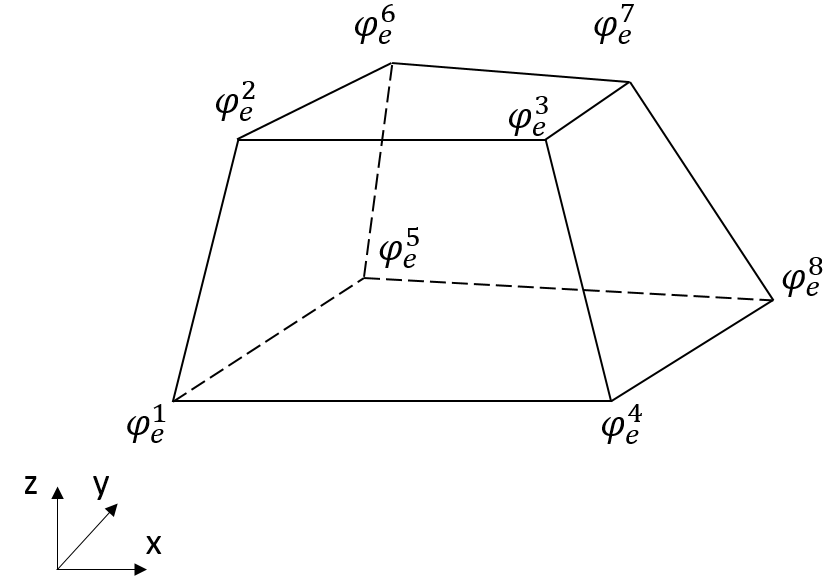
\includegraphics[width=6cm]{chap01/elemento_original_func_forma.png}
\caption{Funções de forma (numeração local).}
\label{fig:elem_func_form_local}
\end{figure}


Considere a numeração local da figura \ref{fig:elem_func_form_local}. Nesse caso, o sobrescrito $e$ nos indica que a numeração que está sendo utilizada é a local do elemento. Considerando, por exemplo, a malha $2\times2\times2$ apresentada em \ref{fig:grid2x2_elem3_vermelho}. O elemento 4 aparece em destaque com os nós pertencentes a ele em vermelho. Nesse caso, comparando com a figura \ref{fig:elem_func_form_local} pode-se associar as numerações da seguinte maneira:

\begin{itemize}
   \item $\varphi^4_1=\varphi_{17}$ em $\Omega^e$
   \item $\varphi^4_2=\varphi_{8}$ em $\Omega^e$
   \item $\vdots$
   \item $\varphi^4_7=\varphi_{14}$ em $\Omega^e$
   \item $\varphi^4_8=\varphi_{11}$ em $\Omega^e$
\end{itemize}




Além disso, definindo $\mathbf{x^e_i} = (x^e_i, y^e_i, z^e_i)$ como as coordenadas do nó $i$ do elemento $e$ e $\Omega^e$ o domínio do elemento $e$.



Define-se como matriz do elemento, a matriz que contem apenas os valores não nulos de $a_e(\phijx,\phiix)$ no elemento. A matriz de um elemento genérico $e$ é mostrada em \ref{eq:matrizelem}.

\begin{equation}
\label{eq:matrizelem}
A^e = \aematelem
\end{equation}


Ainda falta uma definição para o valor as funções de forma. De maneira a interpolar o valor da solução $u^*$ nos nós, as funções $\phiix$ irão satisfazer as seguintes propriedades.

\begin{itemize}
\item \begin{equation}\label{eq:func_cond1}
\varphi^e_i(\mathbf{x}^e_j) = \left\{\begin{matrix} 1, \text{ se i = j} \\  0, \text{ caso contrário} \end{matrix}\right.
\end{equation}
\item \begin{equation}\label{eq:func_cond2}
    \sum_{i=1}^8 \phiix = 1
\end{equation}
\end{itemize}


O fato é que definir tais funções nos domínios $\Omega^e$ é uma tarefa complicada. Além disso, a expressão de $a^e(\phiix,\phijx)$ envolve integrais que são mais complicadas em um domínio {\color{red}``irregular''} como $\Omega^e$.


Assim, para o facilitar a definição das funções de forma e do cálculo das integrais pode-se fazer uma mudança para um elemento base $\xi$ definido em $\Omega^\xi = [-1,1]\times[-1,1]\times[-1,1]$. As variáveis que irão indicar as coordenadas nesse novo domínio são $\xi$, $\eta$ e $\zeta$. As funções de base $N_i$ no elemento base são definidas em $\Omega^\xi$ são apresentadas em \ref{eq:func_base}.

\begin{equation}
\begin{matrix}\label{eq:func_base}
N_1(\xi, \eta, \zeta) = \frac{1}{8} (1-\xi)(1-\eta)(1-\zeta) \\
N_2(\xi, \eta, \zeta) = \frac{1}{8} (1-\xi)(1-\eta)(1+\zeta) \\
N_3(\xi, \eta, \zeta) = \frac{1}{8} (1+\xi)(1-\eta)(1+\zeta) \\
N_4(\xi, \eta, \zeta) = \frac{1}{8} (1+\xi)(1-\eta)(1-\zeta) \\
N_5(\xi, \eta, \zeta) = \frac{1}{8} (1-\xi)(1+\eta)(1-\zeta) \\
N_6(\xi, \eta, \zeta) = \frac{1}{8} (1-\xi)(1+\eta)(1+\zeta) \\
N_7(\xi, \eta, \zeta) = \frac{1}{8} (1+\xi)(1+\eta)(1+\zeta) \\
N_8(\xi, \eta, \zeta) = \frac{1}{8} (1+\xi)(1+\eta)(1-\zeta)
\end{matrix}
\end{equation}

Note que, essas funções satisfazem as duas propriedades apresentadas em \ref{eq:func_cond1} e \ref{eq:func_cond2}.


\begin{figure}[!htbp]
\label{fig:elemento_base}
\centering
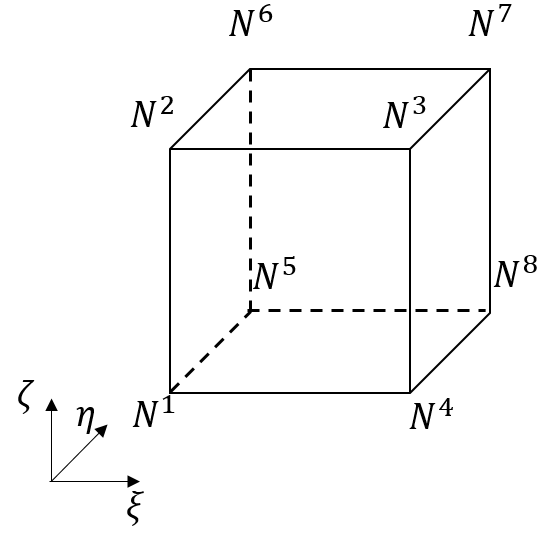
\includegraphics[width=6cm]{chap01/elemento_base.png}
\caption{Elemento base (Domínio $\Omega^\xi$)}
\end{figure}



A associação de um ponto em $\Omega^\xi$ em um ponto em $\Omega^e$ é feito através da equação \ref{eq:isoparametrico}.


\begin{equation}
\label{eq:isoparametrico}
\mathbf{x}(\xi, \eta, \zeta) = \sum_{A=1}^{8} N_A(\xi, \eta, \zeta) \mathbf{x^e_A}
\end{equation}

Assim, pode-se aplicar a mudança de variável na integral da equação \ref{eq:ae_def} para o domínio $\Omega^\xi$.

\begin{equation}
 a_e(\phiix,\phijx) = \omeeint{S^T\phiix D S\phijx} = \omeint[\Omega^\xi]{S^T N^i D S N^j |J|}
\end{equation}


\begin{equation}
 a_e(\phiix,\phijx) = \int^1_ {-1}\int^1_ {-1}\int^1_ {-1}{S^T N^i D S N^j |J|} \text{d}\xi \text{d}\eta \text{d}\zeta
\end{equation}

onde $J$ representa a matriz jacobiana.

\begin{equation}
J = \begin{bmatrix}
\dxi[x]   &  \deta[x]  \\
  \dxi[y] &  \deta[y] 
\end{bmatrix}
\label{eq:jacobiano}
\end{equation}

O valor das derivadas do Jacobiano podem ser obtidas derivando a \ref{eq:isoparametrico}.


\begin{equation}\label{eq:dev_x_xi}
\dxi[x] = \sum^8_{A=1} \dxi[N_A] x^e_A
\end{equation}
\begin{equation}
\deta[x] = \sum^8_{A=1} \deta[N_A] x^e_A
\end{equation}


Pode-se perceber também que os somatórios podem ser transformados como a multiplicação de uma matriz linha por uma matriz coluna transformando, por exemplo, \ref{eq:dev_x_xi} em \ref{eq:dev_x_xi_matriz}.

\begin{equation}\label{eq:dev_x_xi_matriz}
\dxi[x] =
\begin{bmatrix}
 \dxi[N^1]   & \dxi[N^2] & \cdots & \dxi[N^8]
\end{bmatrix}
\begin{bmatrix}
x^1    \\
x^2    \\
\vdots  \\
x^8
\end{bmatrix}
\end{equation}

Com isso, substituindo em \ref{eq:jacobiano} as equações análogas a \ref{eq:dev_x_xi_matriz} para cada uma das entradas do jacobiano é possível obter a equação \ref{eq:jacobiano_prod}.


\begin{equation}\label{eq:jacobiano_prod}.
J = \der
\begin{bmatrix}
x^1 & y^1 & z^1 \\
x^2 & y^2 & z^2 \\
\vdots & \vdots  & \vdots  \\
x^8 & y^8 & z^8 \\
\end{bmatrix}
\end{equation}


